\documentclass[11pt]{ctexart}
\usepackage{graphicx}
\usepackage{amsmath}
\usepackage{booktabs}
\usepackage{cite}
\usepackage{float}
\usepackage{indentfirst}
\usepackage[colorlinks,linkcolor=black]{hyperref}

\setlength{\parindent}{2em}

\usepackage{minted}

\title{OSH详细设计报告\\[2ex]实时文本协作系统}
\author{徐直前 PB16001828\\吴永基 PB16001676\\黄子昂 PB16001840\\金朔苇 PB16001696\\}
\date{\today}
\begin{document}

\maketitle
\tableofcontents

\section{项目概述}
在本项目中,我们参考了有关CRDT的论文,用JavaScript实现了一个基于状态的CRDT,并在此CRDT基础上用JavaScript和Node.js编写前后端,最终实现了一个基于网页端,轻量,能以类似C等语言中
花括号的方式实现块级的权限控制,并且能够对Markdown语法支持以及实现实时预览,也具有一定的鲁棒性。其主要特征如下:
\begin{itemize}
    \item 基于CRDT实现,具有很好的可伸缩性;
    \item 采用纯JavaScript编写,为网页端应用;
    \item 使用Node.js作为后端,利用npm包管理器可以很方便地完成部署;
    \item 支持Markdown,并支持实时预览;
    \item 能实现精确到块级的权限控制,管理员可以指定某块内容只能由某个用户编辑,同时也可以指定一个公共的编辑区域;
    \item 具备高度可再开发性,基于本项目可以实现更高级的实时文本协作应用。
\end{itemize}

目前权限管理采用免登陆的方式,第一个登陆网页的人即为管理员(admin),此后登陆的人都为普通用户(guest)。仅有管理员拥有全部权限,
可以控制普通用户的编辑权限。而普通用户不能进行权限的编辑。
管理员权限也会动态转移。当当前管理员离线时,管理员权限会即可转移到第一个guest上。
这种免登陆的权限控制实施方案极适用于一个团队在同一个局域网内进行实时协作。当然,也可以维护一个相应的用户数据库,实现用户名密码登陆的用户管理方式,
此部分内容在本项目基础上很容易扩展,而且与实时文本协作的核心技术难题无关,故没有实现该种方式。

我们将本项目部署在了一台腾讯云服务器上,并且也在结题汇报时进行了现场互动演示,实现了很好的效果。
\begin{figure}[ht]
    \begin{center}
    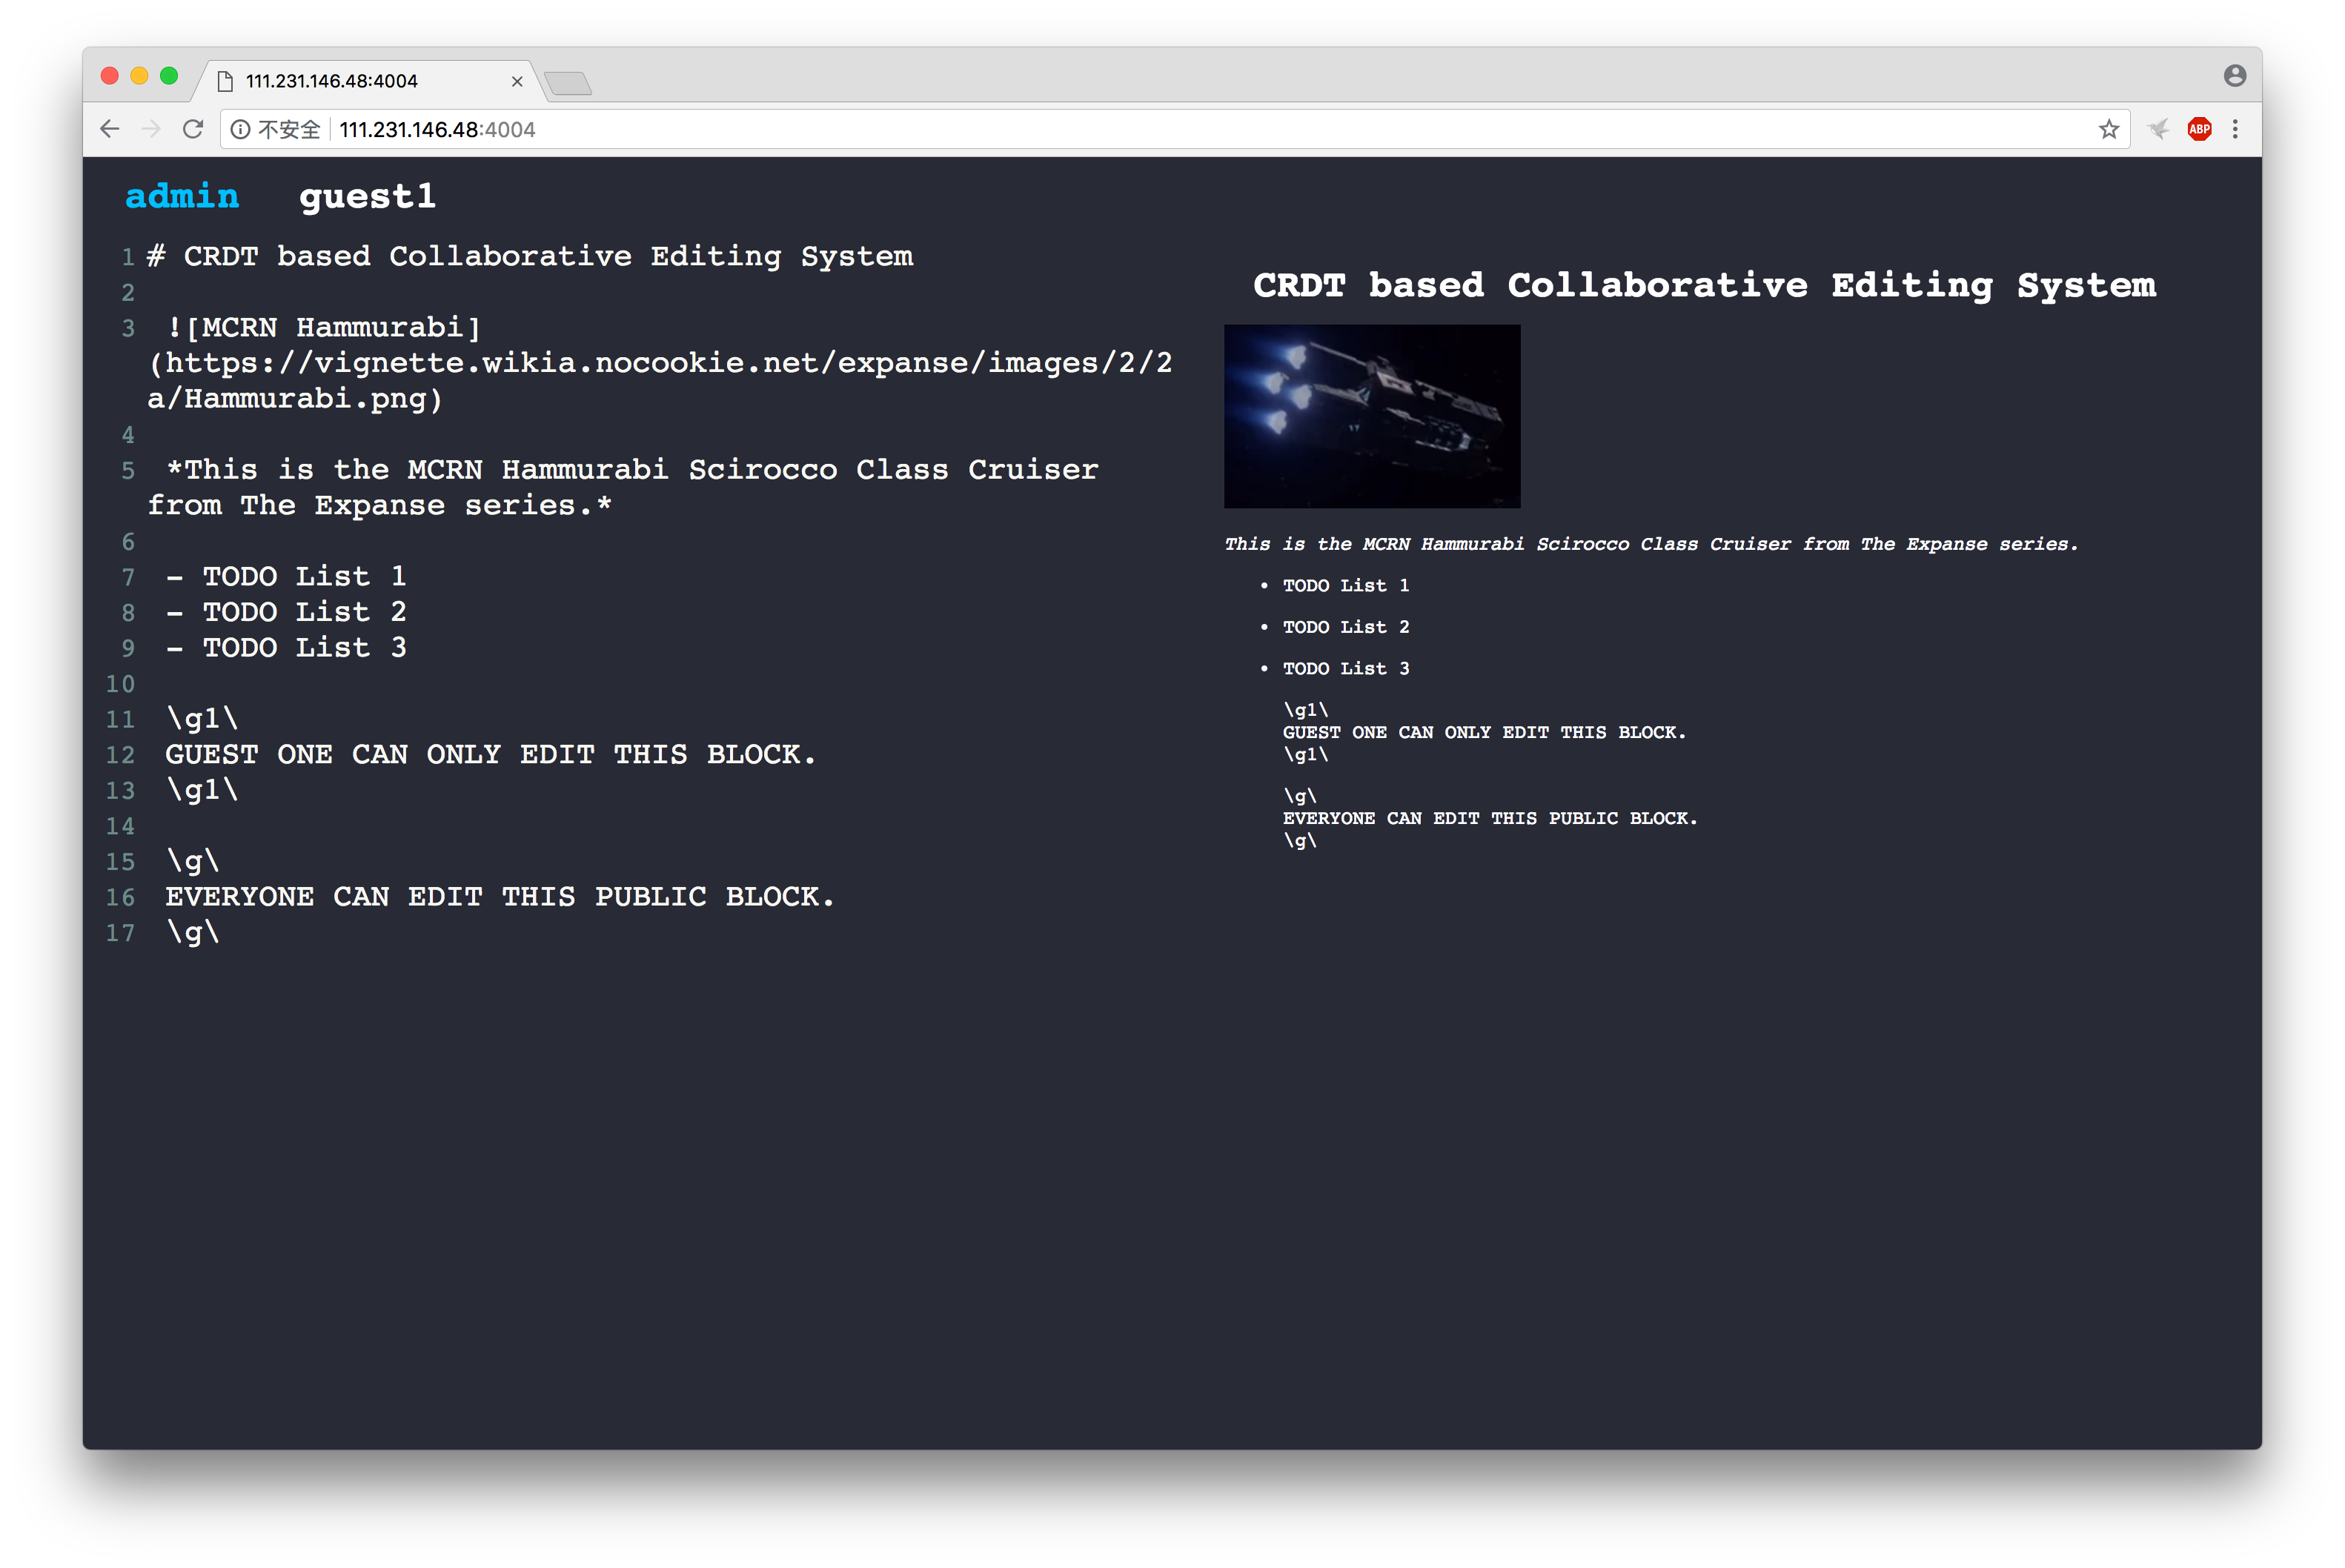
\includegraphics[width=\textwidth]{figures/demo.png}
    \caption{最终实现效果}
    \end{center}
\end{figure}
\section{背景知识}
本部分内容将介绍与此项目相关的背景知识,其部分内容在调研报告和可行性报告中也有所介绍,在此也对其中的关键内容进行一下回顾。
\subsection{实时文本协作的技术难点}
实时文本协作从用户层面来说看似十分简单,然而其面对的技术难题却是相当巨大的。业界在此问题上也进行了几十年的研究,最终也才在近些年来诞生了像Google Docs这样较为
完善的实时文本协作系统。其主要的难点在于解决不同用户的数据副本之间的同步问题。  

通常在这种高交互性的网络应用中,为了隐藏网络延时对用户体验带来的影响,我们要在每个客户端上
保存一个本地的用户副本。每个用户的操作都直接在本地数据副本上执行,这样本地的操作就不会受到网络延时的影响,用户能获得很好的本地响应性。
然而,这样的方式也会带来问题。需要设计一种机制维持各个用户的数据副本之间的一致性。如果用户的副本出现了不一致的情况,
那么显然会导致灾难性的后果。


\nocite{*}
\bibliographystyle{plain}
\bibliography{ref}
\end{document}